\documentclass[11pt]{article}
\renewcommand{\baselinestretch}{1.05}
\usepackage{amsmath,amsthm,verbatim,amssymb,amsfonts,amscd, graphicx}
\usepackage{graphics}
\usepackage{braket}
\topmargin0.0cm
\headheight0.0cm
\headsep0.0cm
\oddsidemargin0.0cm
\textheight23.0cm
\textwidth16.5cm
\footskip1.0cm
\theoremstyle{plain}
\newtheorem{theorem}{Theorem}
\newtheorem{corollary}{Corollary}
\newtheorem{lemma}{Lemma}
\newtheorem{proposition}{Proposition}
\newtheorem*{surfacecor}{Corollary 1}
\newtheorem{conjecture}{Conjecture}
\newtheorem{question}{Question}
\theoremstyle{definition}
\newtheorem{definition}{Definition}
\renewcommand\thesubsection{\alph{subsection}}
\usepackage[framed,numbered,autolinebreaks,useliterate]{mcode}

% something NOT relevant to the usage of the package.
\usepackage{url,textcomp}
\setlength{\parindent}{0pt}
\setlength{\parskip}{18pt}
\title{\texttt{mcode.sty} Demo}
\author{Florian Knorn, \texttt{florian@knorn.org}}
\usepackage{listings}

 \begin{document}
 
\title{IVR 1}
\author{Katrina Yankova 
% \newline
and 
% \newline
Francisco Vargas}
\maketitle

\section{Introduction}
The following report aims to detail how several vision techniques are employed to extract features and classify a deck of playing cards. 
\newline
\newline
As an initial stage we 
employed edge detection techniques to detect the
bounding box of the card and crop it in order to
eliminate the back ground as much as possible.

Furthermore we employed auto-calibrating threshold based segmentation to extract the bounding boxes of the features within the cropped cards. The final stage consisted in extracting image signatures and complex moments, allowing us to create feature vectors for classification via Naive Bayes. The classification via Nave Bayes yielded excellent results due to the high quality feature extraction and astute noise reduction techniques employed throughout this practical. 
\newline
\newline
We used a great chunk of material from the course slides, the lab code and inbuilt matlab functions; This being said we did not apply at any time the 'black box' of employing things without understanding. In to depth research was applied for every inch of this practical along with a bit of hacking and creativity, which we hope to justify in the following chapters. 

\section{Methods}
\subsection{Bounding Box and Image Cropping}
Since the cards have well defined edges it seemed like a good idea to detect these edeges
employ its connected region as a bounding box and crop out the original greyscale card.
\newline
\newline
The laplacian takes the general definition of $\nabla^{2} = \sum_{i=1}^{n}\frac{\partial^2}{\partial x_{i}}$ which for our case we are only interested in two dimensions thus $n=2$.
The continuous Laplacian of the gaussian kernel is defined as follows:
\begin{equation*}
\nabla^{2}\mathcal{N}(\underline{x};\sigma)= -\frac{1}{\pi \sigma^{2}}\left[ 1 -\frac{x^{2} + y^{2}}{2\sigma}\right]e^-\frac{x^{2} + y^{2} }{2\sigma}
\end{equation*}
This formula is used to aproximate a discrete kernel, we have the following exammple:
\[
\begin{pmatrix}
  0 & 1 & 0 \\
  1 & -4 & 1 \\
  0 & 1 & 0
 \end{pmatrix}
\]
The kernel is applied via 2D convolution with the image. In a sense one may picture this procedure as first convolving with a Gaussian and then applying the laplacian which aims to find the areas of rapid change in other words the edges.
\newline
\newline
\begin{lstlisting}
I = rgb2gray;
% binary image yielding 
bw = edges(I,'log');
% remove noise using open
% open is a mix of both erosion and dilation
bw = bwareaopen(bw,15);
% lable connected regions
lables = bwable(bw);
%{ obtain properties for lables
such as BoundingBox for example
Which is later used to crop the 
greyscale of the original 
image (normalized by rgbnorm.m)
%}
properties = regionprops(lables, 'all');
\end{lstlisting}
% \newline
\subsection{Thresholding the Features}
Before thresholding the features the histograms 
we inspected the histograms and by a method of trial and error we devised the location of the suits within the cropped card and tweaked the 
findthresh.m algorithm to target the correct
valley. It is important to note that our gray
intensity is conveniently between 0 and 1 due to a witty cast. The histograms were smoothed before iteration over then and as we went through the project:
\begin{center}
        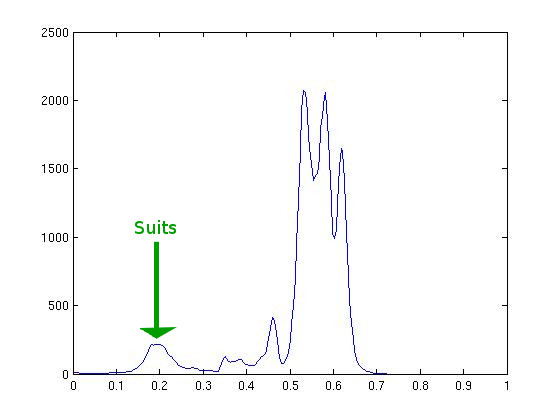
\includegraphics[scale=0.7]{suit.jpg}
\end{center}
The tiny peaks within a bigger peak were sources of distortion and mis-calibration thus we increased the size of the Gaussian kernel to blur these out more when convolving. Empirically we determined the kernel size to be 1x40 and it yielded histograms of the following form:
\newline\newline
INSERT IMAGE

After thresholding we removed small area (less than 150 px) elements and used the following morphological transform.  
\begin{lstlisting}
bw = bwmorph(bw,'mayority');
\end{lstlisting}
An additional noise removal technique (for long rectangles) was to look at the mayor axis to minor axis ratio and check that
it is not greater than 3. If it was greater than 3 we removed it. All these constants for removal were determined empirically
throughout the practical.

We then found the bounding boxes for the remaining elements and cropped the original image (gray scaled) for each single one of these features. On every new cropped feature the following was applied to threshold
\begin{lstlisting}[mathescape]
% Inverted global threshold 
% graytrhesh computes global
% threshold level.
% we invert this to extract the suit
bw = $\text{\texttildelow}$im2bw(Icropped,graytrhesh(I));
\end{lstlisting}
resulting in: 
 INSERT PICTURE HERE
\subsection{Construction of Feature Vector for Suit classification}
For every suit symbol in each card we generated a feature vector. For example 2 of diamonds would ideally yield 4 feature vectors. The feature vectors consisted of 4 dimensions compactness, the first two rotation and scale invariant moments and the average of 
the normalized red channel of the suit which is closest to the center. The reasoning behind this is that the region detected closest to the center should be a suit (which yields a lot more pixels with color than a number); The closer you are to the center of the card the less likely the region is noise (again this is based on empirical evidence but also some common sense).
\[
\underline{x}_{feature} = \braket{\enskip compactness, \enskip ci_{1}, \enskip ci_{2}, \enskip \text{\bf mean}(red\_channel) \enskip}
\]
The other $ci_{k}, \enskip k \in [3,7]$ yield significantly small values along the order of magnitude of $10^{-5}$ and produced no changes in the classification problem, hence they were discarded due to their poor discrimination power. The normalization of the red channel before averaging accounts for dealing with brightness. We chose not to build two different classifiers since it seems quite hacky to identify red and black by assuming there normalized rgb values are approximately 0.3333 and 0.6 (which they are nonetheless when averaging within the bounding box of the suits these values may be averaged out resulting in confusion). 
\subsection{Counting the number}
Out of 480 features (+ approximately 30 incorporated later) the detection of the features was perfect it drew the bounding box  on all features and no noise created any issues. This fact lead us to deciding that counting the number of regions and subtracting 4 was the correct decision for determining the number of the card. We opted out of naive Bayes since it is almost impossible to differentiate between 9 an 6 since they are exactly the same. A possible solution to classification via machine learning would be to compute the global moments of the card and incorporate them as dimensions since the 6 has less symbols than 9 the global moments and other global signatures could have relatively high discrimination powers.


% \subsecion{}
\end{document}